\showboxdepth=\maxdimen
\showboxbreadth=\maxdimen

\documentclass [ngerman]{mucproc}
%%%%%%%%%%%%%%%%%%%%%%%%%%%%%%%%%%%%%%%%%%%%%%%%%%%%%%%%%%%%%%%%%%%%%%%%%%%%%%%%%%%%%%%%%%%%%%%%%%%%%%%%%%%%%%%%%%%%%%%%%%%%%%%%%%%%%%%%%%%%%
%Quellen
\bibliography{DLN.bib}
%%%%%%%%%%%%%%%%%

%%%%%%%%%%%%%%%%%
%Für Tabellenbeispiel
\usepackage{tabularx}
\usepackage{booktabs}
%%%%%%%%%%%%%%%%%

\usepackage[table,gray]{xcolor}

%%%%%%%%%%%%%%%%%
%Nur wegen der Codebeispiele notwendig

%%%SyntaxHighlighting: Needs pygmentize installed and -shell-escape set. See minted-documentation for for information.
\usepackage{minted}
\setminted{bgcolor=black!10,tabsize=4}
\NewDocumentCommand{\inlinemint}{O{}mv}{\mintinline[#1]{#2}{#3}}
\usemintedstyle{friendly}

\usepackage{listings}

%%Fallback wenn minted nicht konfiguriert ist
\usepackage{verbatim}% http://ctan.org/pkg/verbatim
\newenvironment{minted}[2][]{\endgraf\verbatim}{\endverbatim}
\NewDocumentCommand{\inlinemint}{omv}{\texttt{#3}}

%Symbol-Font: Sonst sind die Symbolschriftarten nicht voll skalierbar
\usepackage{unicode-math}
%\setmathfont{Latin Modern Math}
%%%%%%%%%%%%%%%%


%%%%%%%%%%%%%%%%%%%%%%%%%%%%%%%%%%%%%%%%%%%%%%%%%%%%%%%%%%%%%%%%%%%%%%%%%%%%%%%%%%%%%%%%%%%%%%%%%%%%%%%%%%%%%%%%%%%%%%%%%%%%%%%%%%%%%%%%%%%%
\begin{document}
	\title{MPPT-Laderegler Monitoring über Http Requests via ESP32 }%Tragen Sie hier den Titel Ihrer Einreichung ein.
	\author{Harun Dastekin s0551006\thanks[HTW Berlin]{Studiengang: Angewandte Informatik, Drahtlose Netze}}
	\email{Harun.Dastekin@Student.HTW-Berlin.de}
	
\maketitle
%%%%%%%%%%%%%%%%%%%%%%%%%%%%%%%%%%%%%%%%%%%%%%%%%%%%%%%%%%%%%%%%%%%%%%

%%%%%%%%%%%%%%%%%%%%%%%%%%%%%%%%%%%%%%%%%%%%%%%%%%%%%%%%%%%%%%%%%%%%%	
\begin{abstract}
Dieser Text behandelt zwei unterschiedliche Methoden zur zeitlichen Optimierung des Stromverbrauches und der Stromerzeugung in privaten Haushalten.

Diese Anwendung erlaubt es dem Nutzer von überall her seine Solaranlage zu überwachen.
\end{abstract}	
%%%%%%%%%%%%%%%%%%%%%%%%%%%%%%%%%%%%%%%%%%%%%%%%%%%%%%%%%%%%%%%%%%%%%%%%%%%%%%%%%%%%%%%%%%%%%%%%%%%%%%%%%%%%%%%%%%%%%%%%%%%%%%%%%%%%%%%%%%%%
	
\section{Einleitung}
	Die Solaranlage besteht aus drei Komponenten. Der Solaranlage die eine unbestimmte und variable Spannung liefert. Der Batterie die eine stabile Spannung 

	In unserer heutigen Zeit ist ein Zugang zu Stromanschlüssen maßgeblich entscheidend für den Komfort. Oft liegt aber eine Steckdose nich genau dort wo man sie gerne braucht. Abhilfe sorgen hierbei Solaranlagen die im besten Fall im Inselbetrieb arbeiten können. Mit anderen worten ein abgeschlossenes Energiesystem mit Energiezufuhr, Energiespeicher und einer möglichkeit sie zu diese Energie zu nutzen. Und um die Energiezufuhr ideal zu gestalten braucht gibt es einige Faktoren die dies beeinflussen. Darunter auch die Regulierung der Energiezufuhr und des Energiespeicher mit dem Verbrauch. D.h. eine Solarbatterie darf weder überladen noch tiefenentladen werden. Es muss eine Ladekurve geben, die den Ladevorgang reguliert. 
	
Ein erster Schritt wäre es diese Anlage zu überwachen und darauf geht diese Projektarbeit ein.

%%%%%%%%%%%%%%%%%%%%%%%%%%%%%%%%%%%%%%%%%%%%%%%%%%%%%%%%%%%%%%%%%%%%%%%%%%%%%%%%%%%%%%%%%%%%%%%%%%%%%%%%%%%%%%%%%%%%%%%%%%%%%%%%%%%%%%%%%%%%
\newpage
\section{Haupteil}

	\subsection{Bauteile}
		

	Die Solaranlage besteht im Grunde genommen aus drei bzw. vier Bestandteilen. Einer 12V Batterie \ref{fig:Batterie}, einem Laderegler \ref{fig:Laderegler} und dem Photovoltaikmodul \ref{fig:Solarmodul} und gegebenenfalls dem Verbraucher.

\begin{figure}
   \begin{minipage}[b]{.4\linewidth} % [b] => Ausrichtung an \caption
      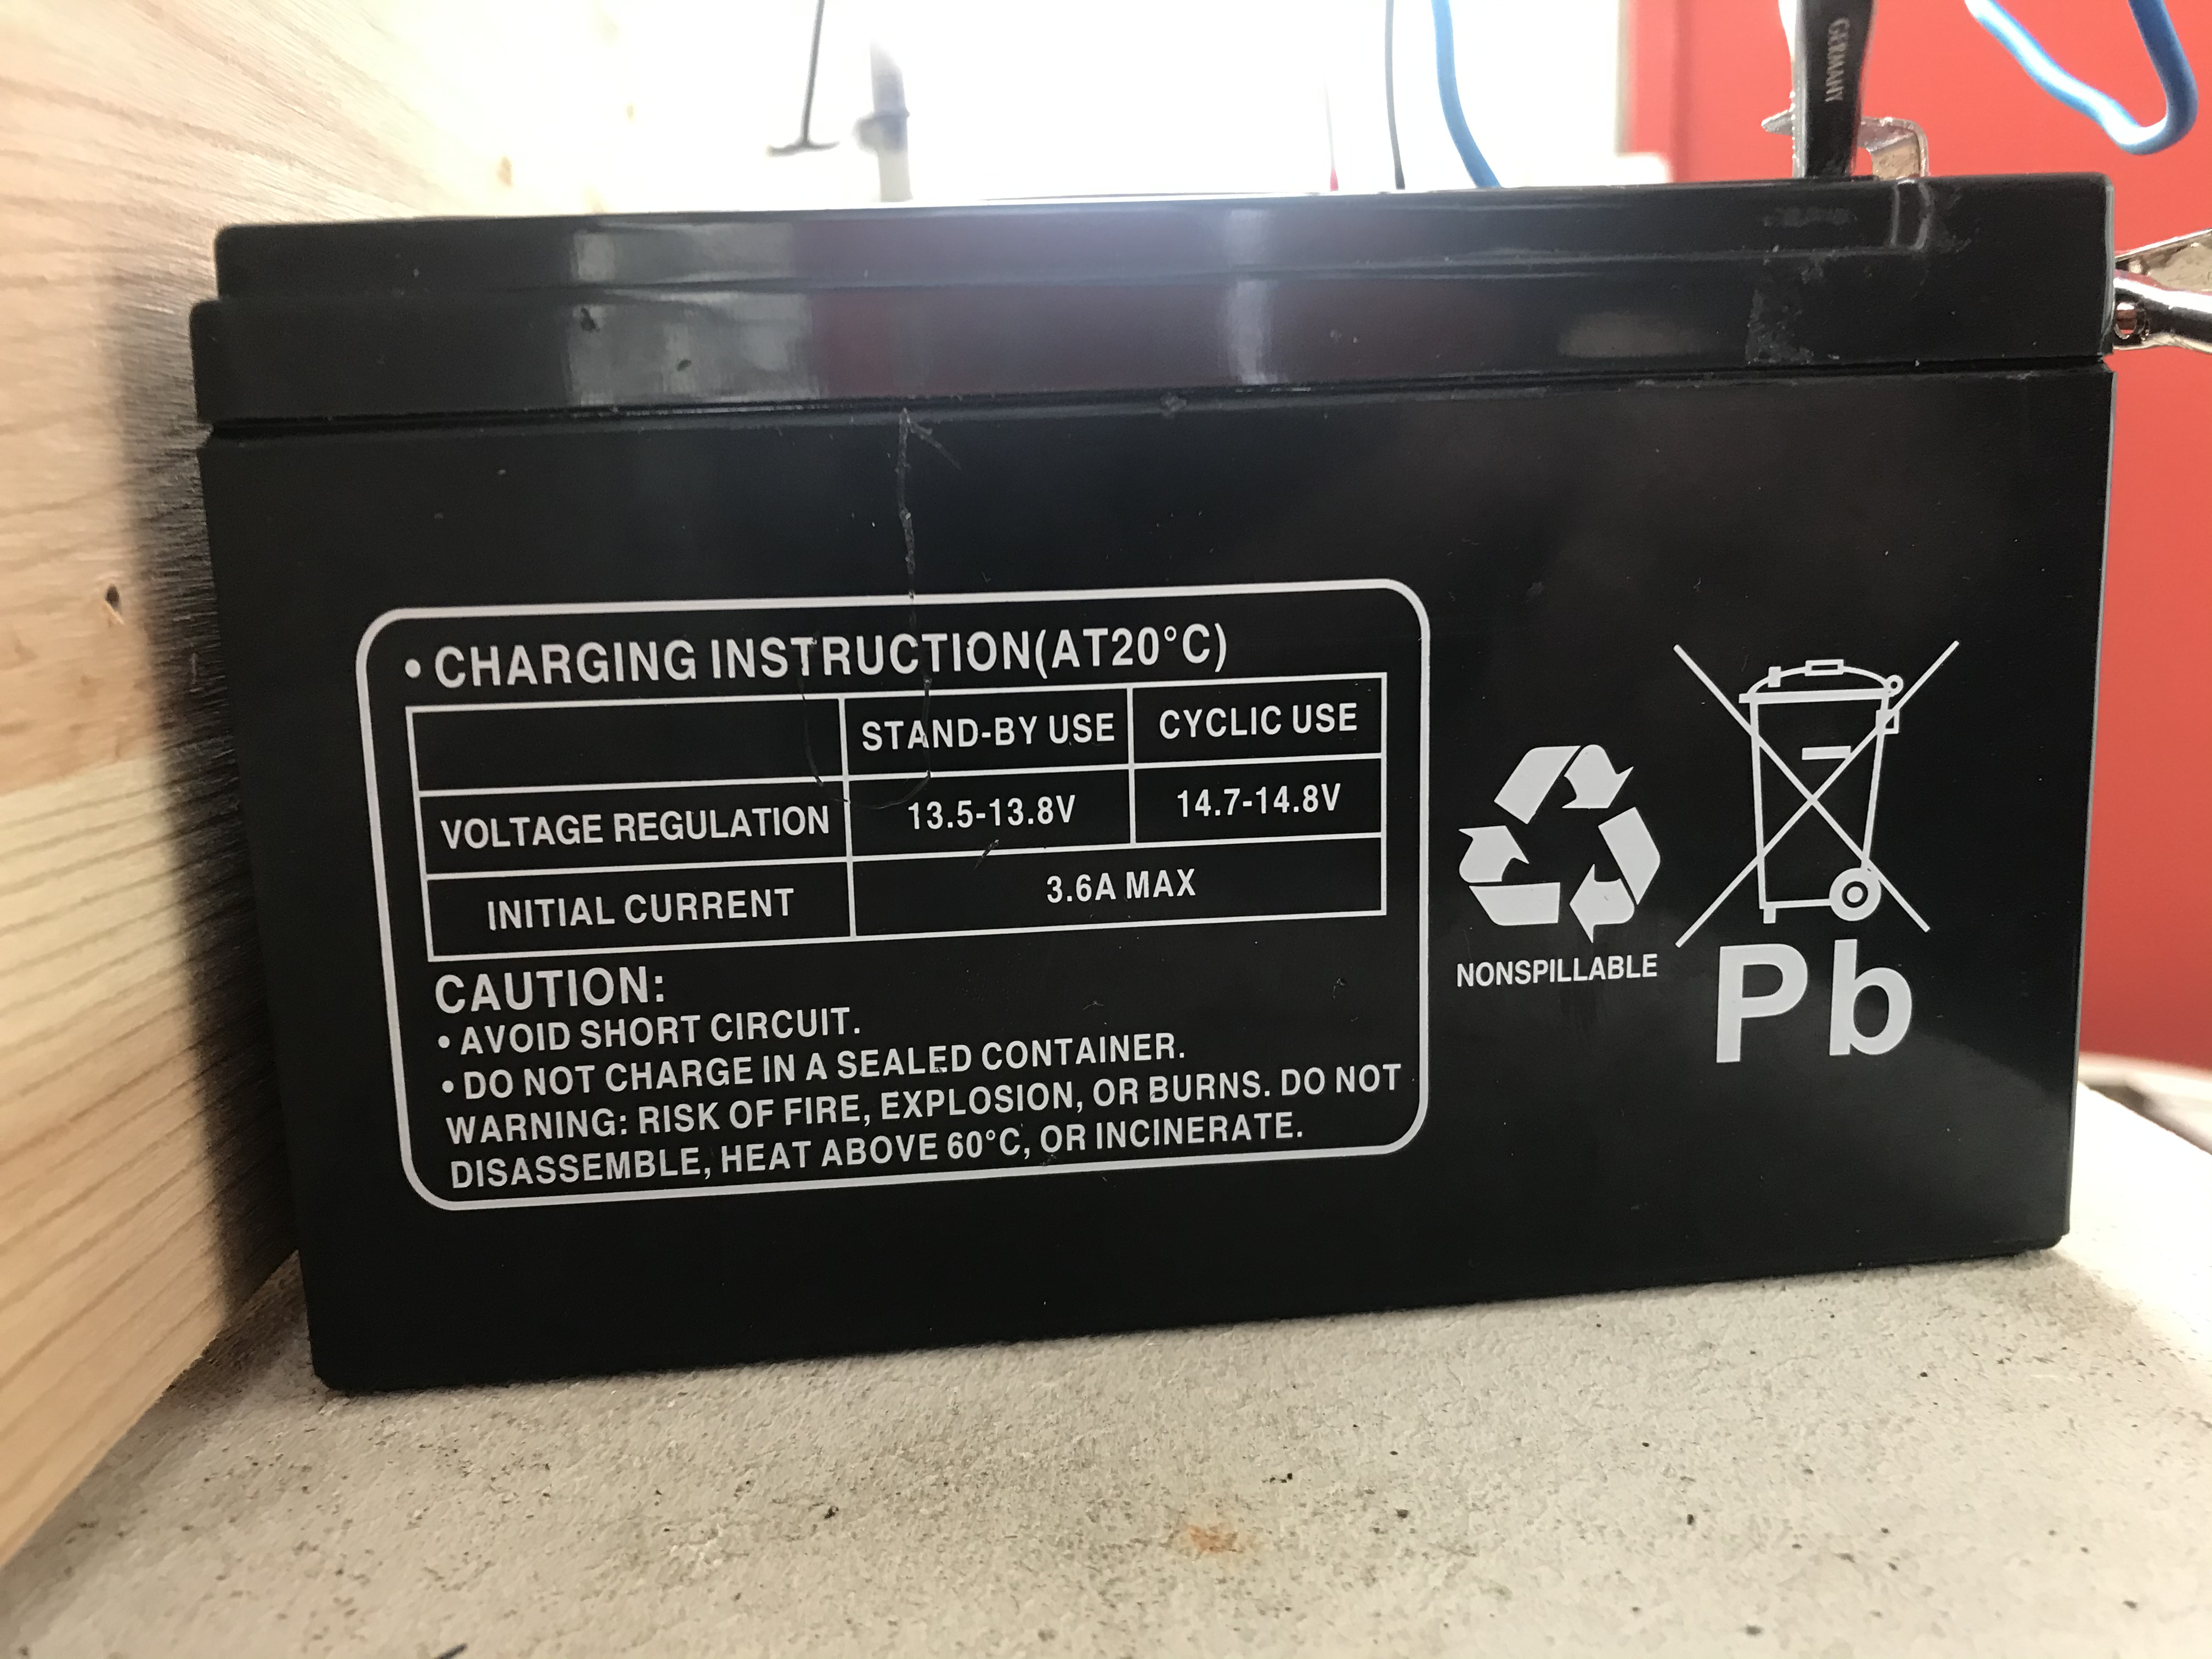
\includegraphics[width=\linewidth]{Bilder/Dokubilder/Batterie.jpg}
      \caption{12V Batterie}
      \label{fig:Batterie}
   \end{minipage}
   \hspace{.1\linewidth}% Abstand zwischen Bilder
   \begin{minipage}[b]{.4\linewidth} % [b] => Ausrichtung an \caption
      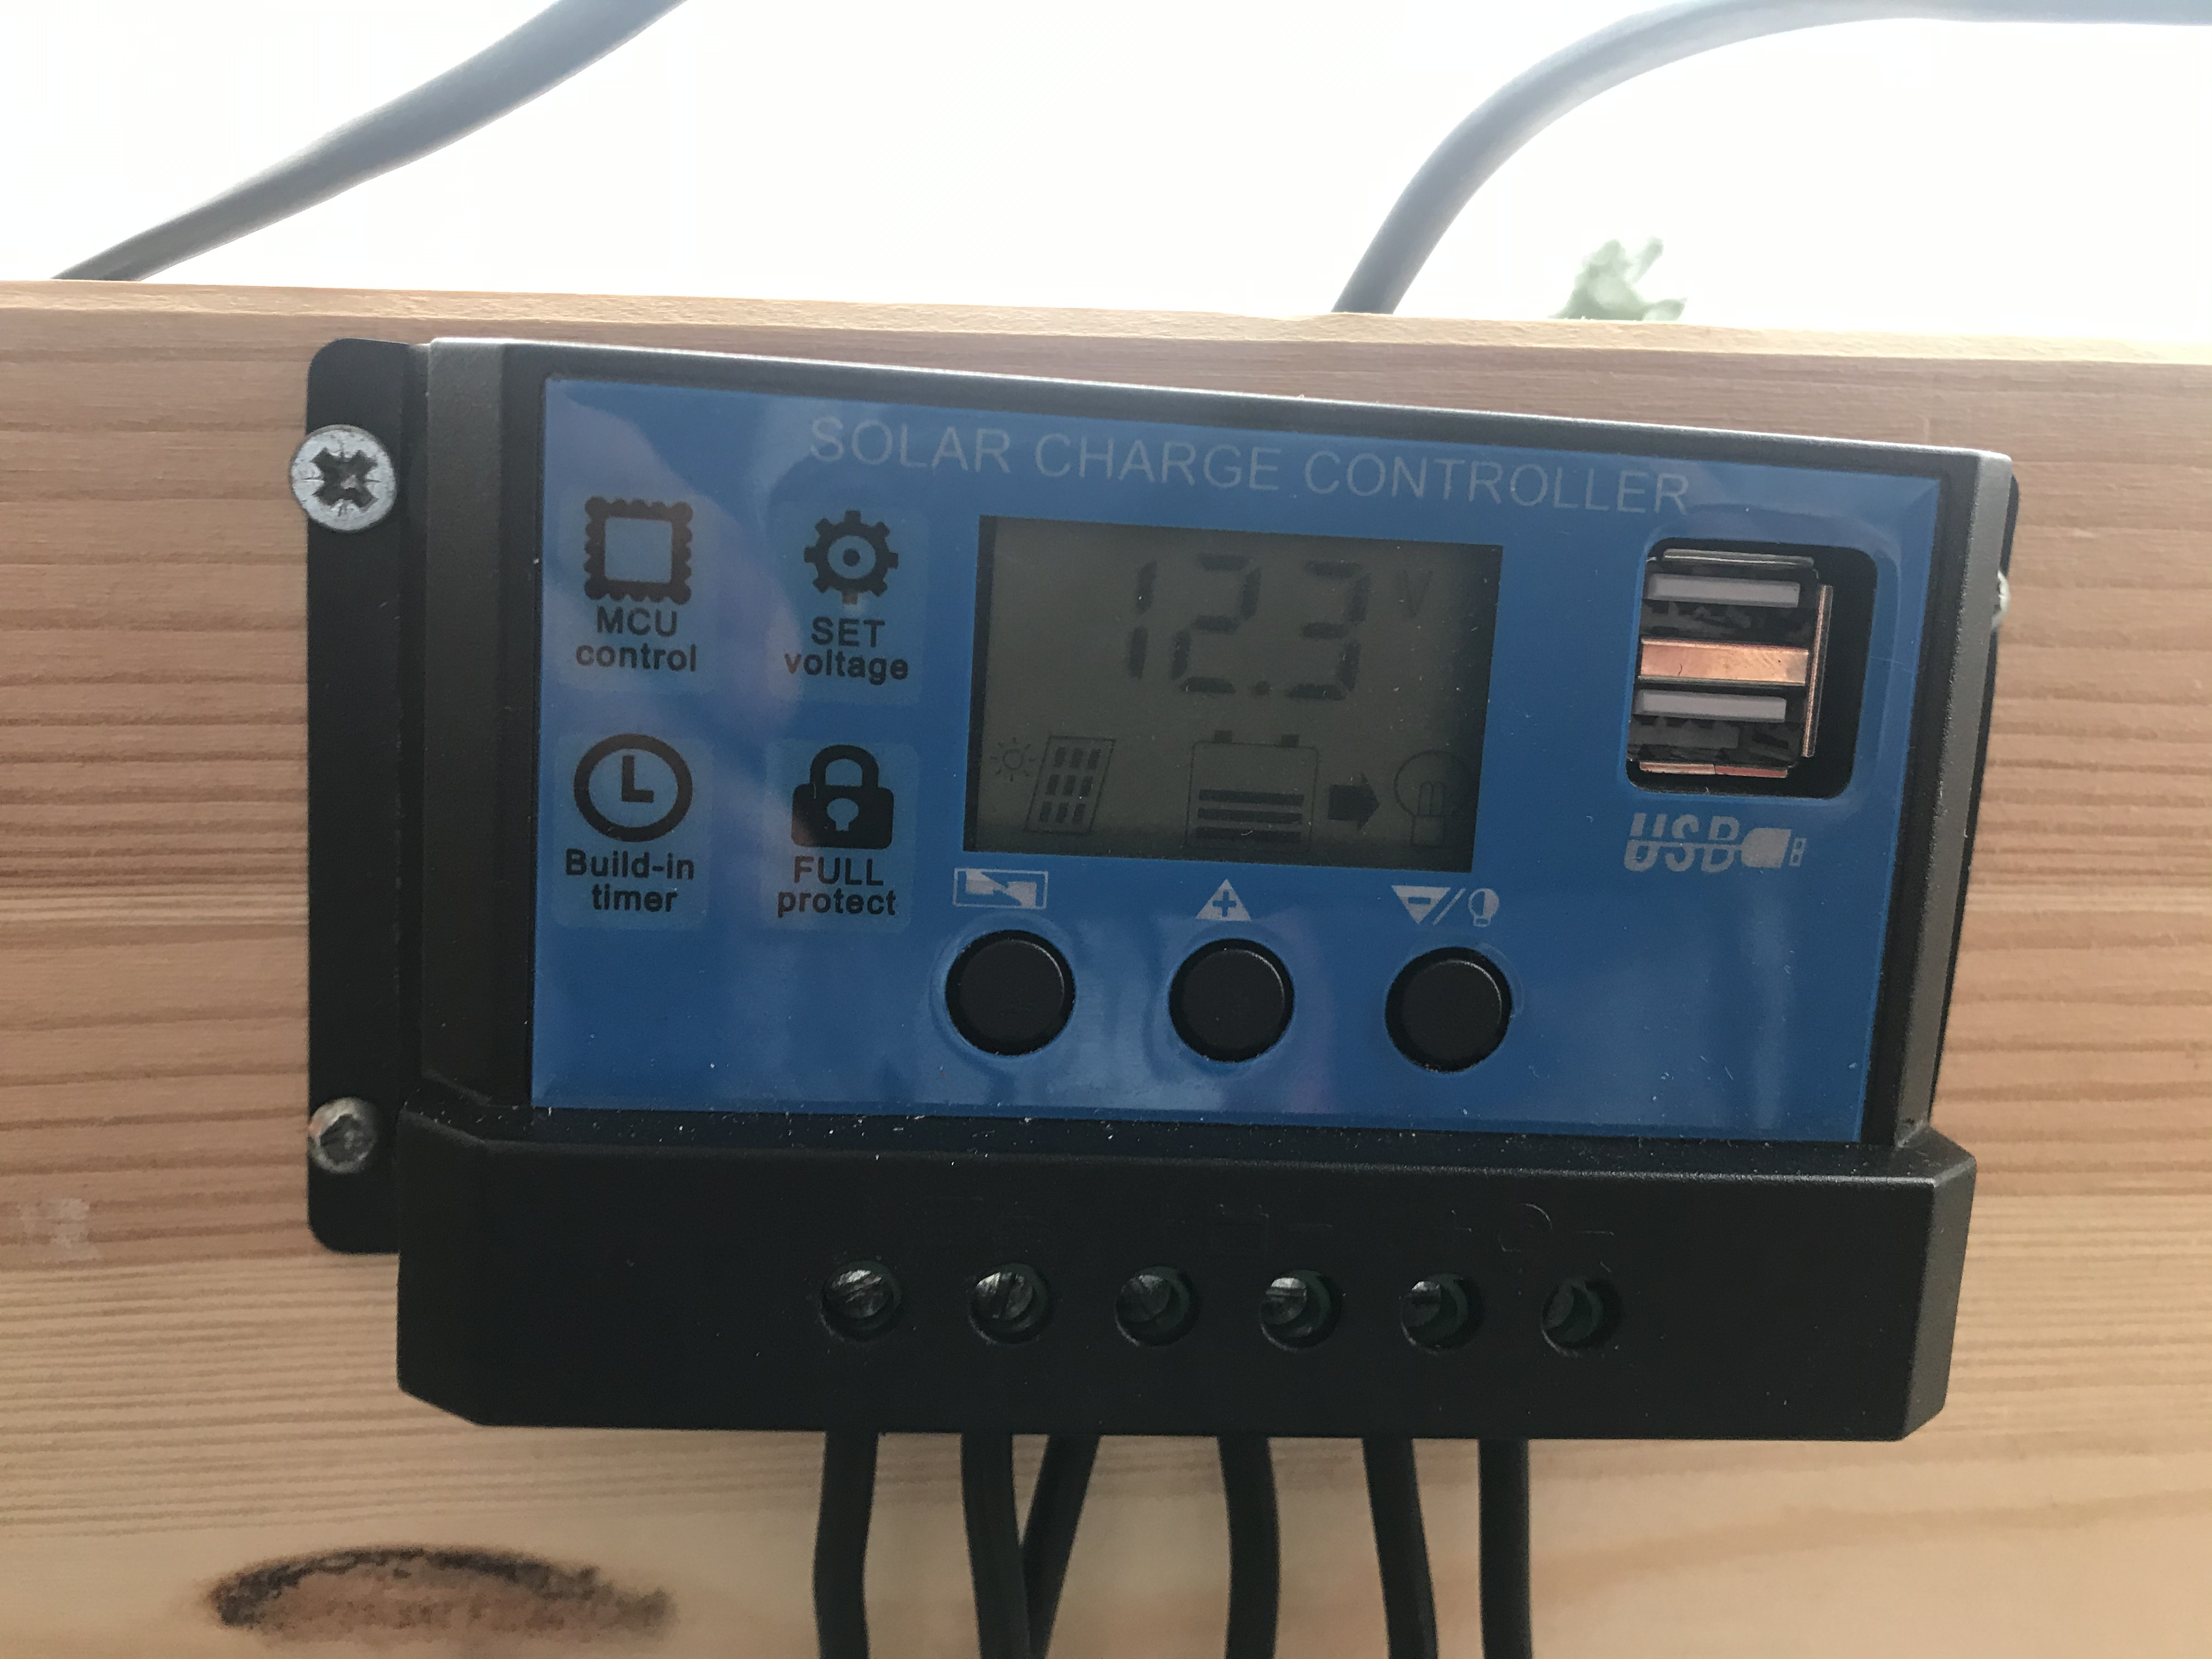
\includegraphics[width=\linewidth]{Bilder/Dokubilder/Controller.jpg}
      \caption{Solar Laderegler}
		\label{fig:Laderegler}
   \end{minipage}
\end{figure}

\begin{figure}
   \begin{minipage}[b]{.4\linewidth} % [b] => Ausrichtung an \caption
      \includegraphics[width=\linewidth]{Bilder/Dokubilder/PVKlein.jpg}
		\caption{kleines PV Modul}
		\label{fig:Solarmodul}
   \end{minipage}
   \hspace{.1\linewidth}% Abstand zwischen Bilder
   \begin{minipage}[b]{.4\linewidth} % [b] => Ausrichtung an \caption
      \includegraphics[width=\linewidth]{Bilder/Dokubilder/LadereglerAlt.jpg}
			\caption{Verbraucher}
			\label{fig:Verbraucher}
   \end{minipage}
\end{figure}





%	\begin{figure}
%		\centering
%		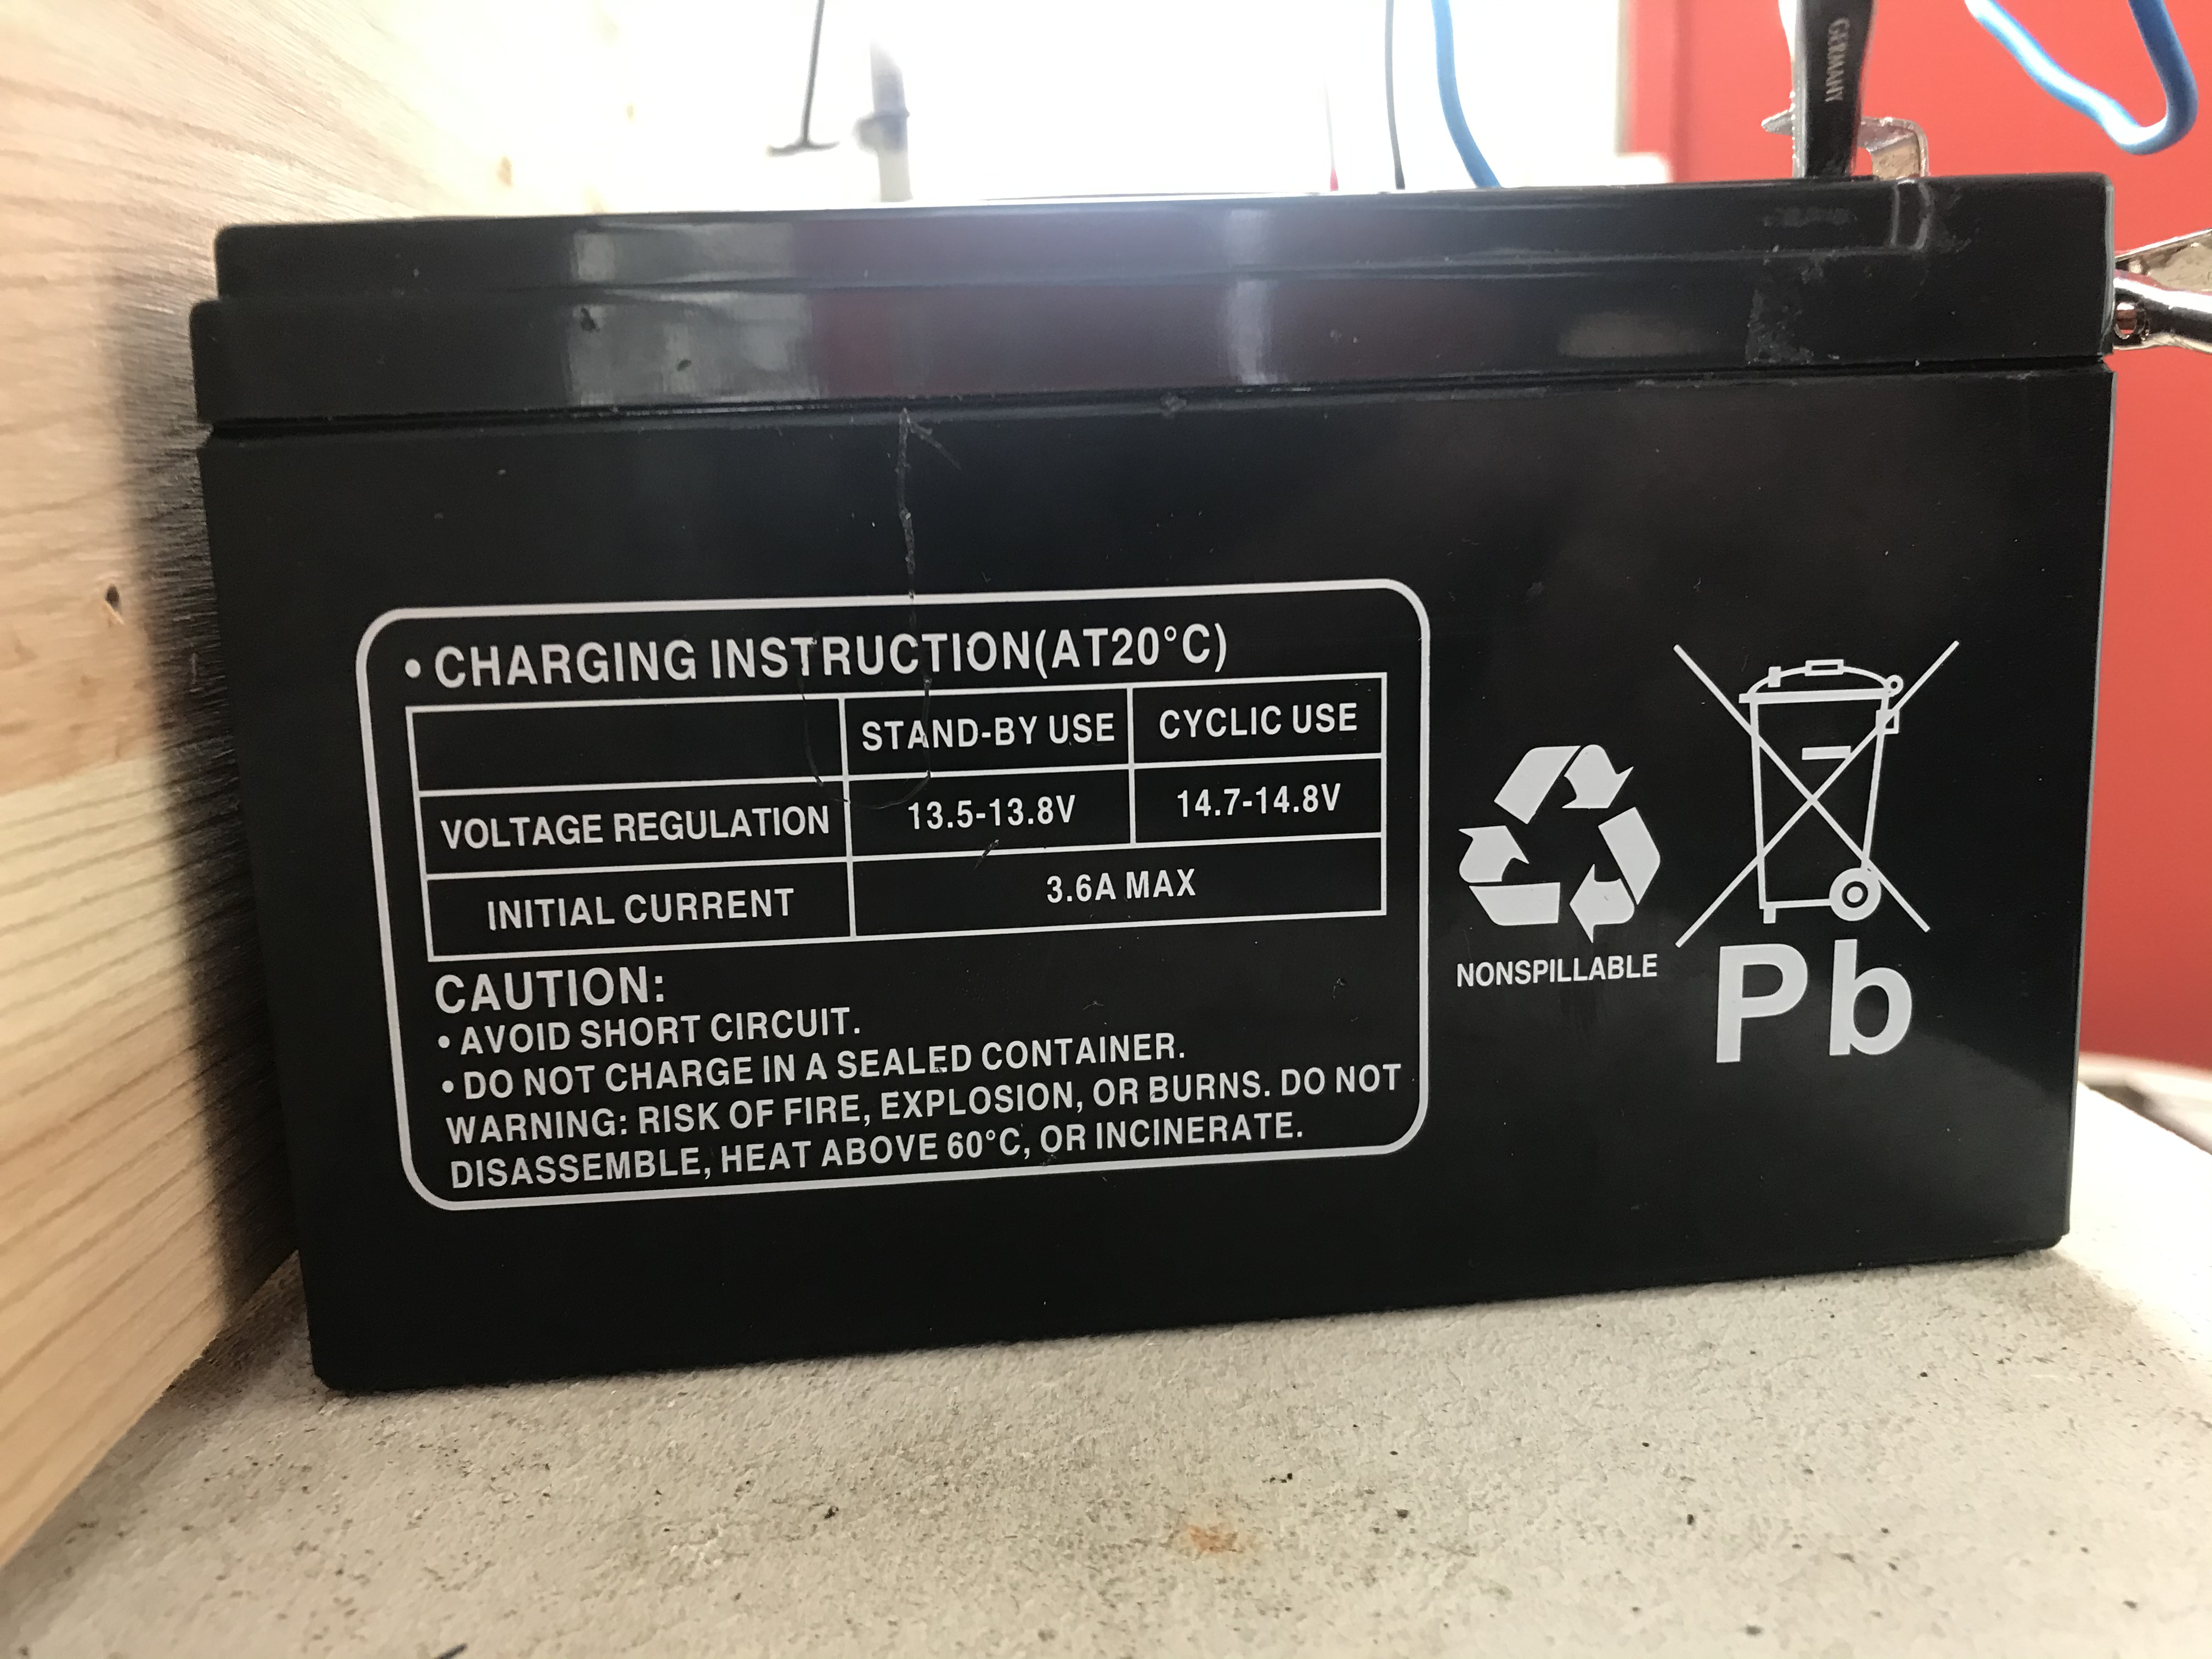
\includegraphics[width=1\linewidth]{Bilder/Dokubilder/Batterie.jpg}
%		\caption{12V Batterie}
%		\label{fig:Batterie}
%	\end{figure}	
%		
%	\begin{figure}
%		\centering
%		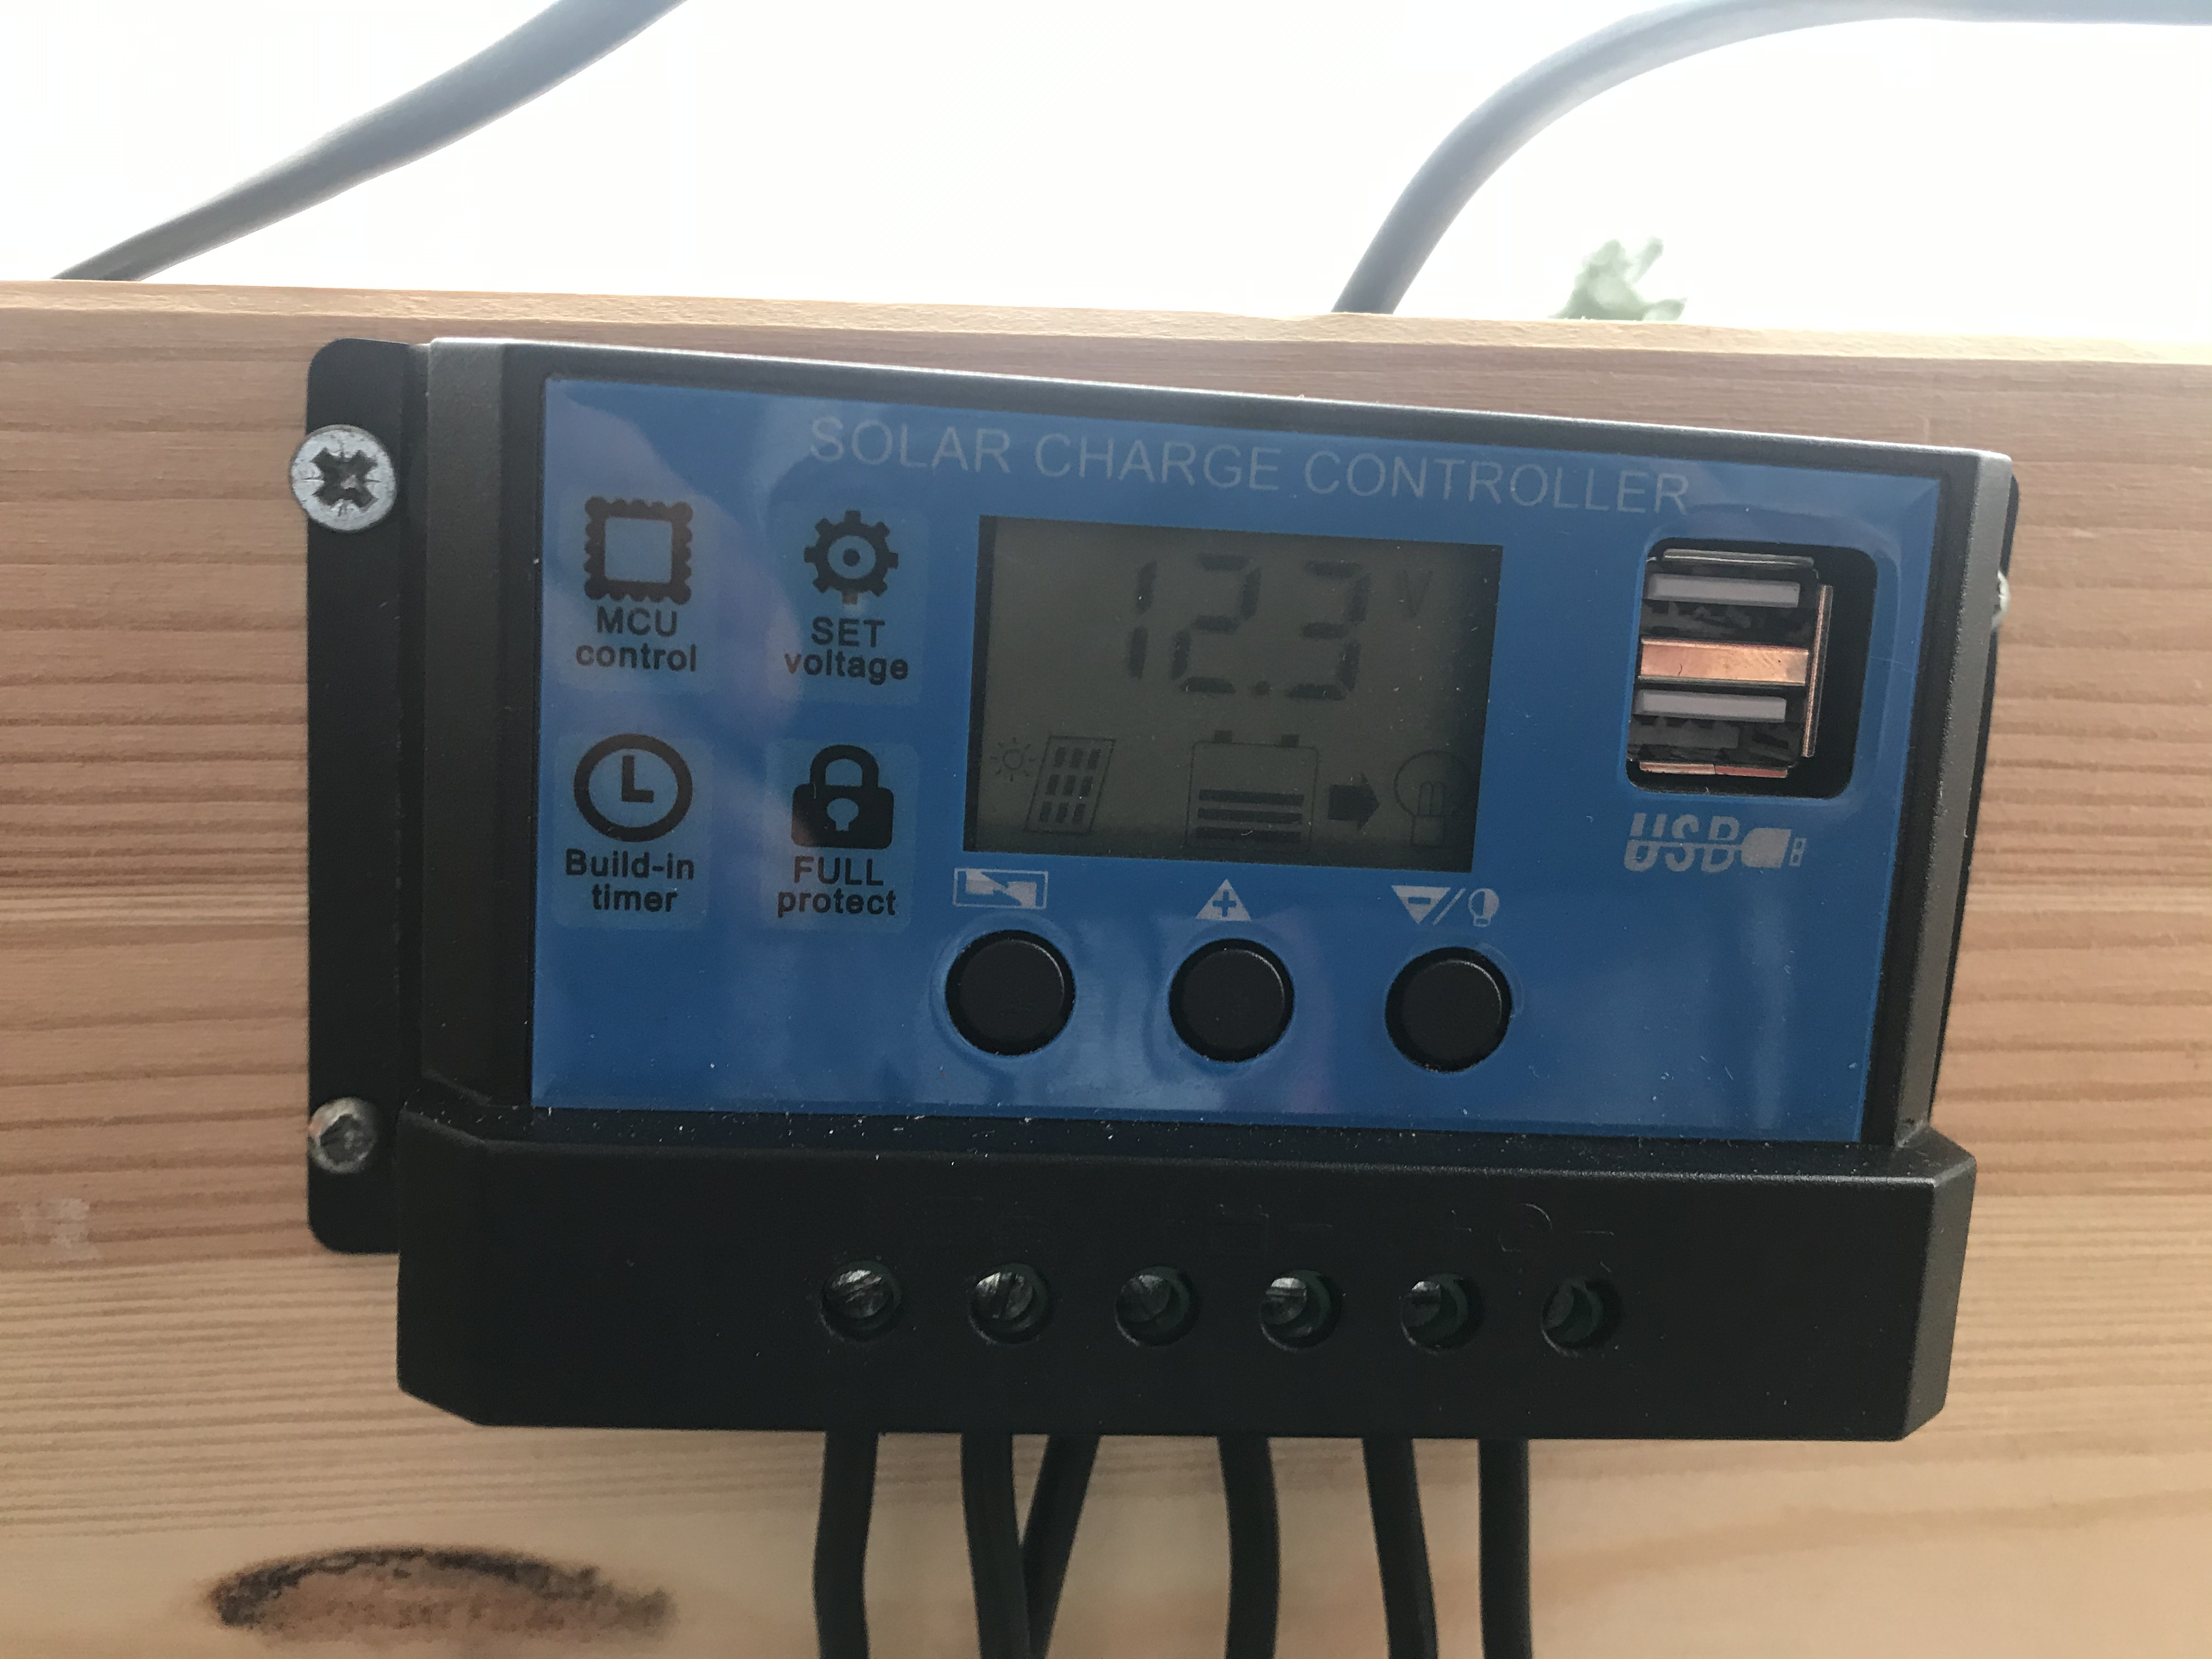
\includegraphics[width=1\linewidth]{Bilder/Dokubilder/Controller.jpg}
%		\caption{Solar Laderegler}
%		\label{fig:Laderegler}
%	\end{figure}
%		
%	\begin{figure}
%		\centering
%		\includegraphics[width=1\textwidth]{Bilder/Dokubilder/PVKlein.jpg}
%		\caption{kleines PV Modul}
%		\label{fig:Solarmodul}
%	\end{figure}
	
	
	
	
	Das Monitoring System setzt an 4 Punkten ein. Die Spannung des Photovoltaikmoduls sowie der Batterie werden jeweils mit einem Spannungssensormodul gemessen. 
	
	Die Ströme durch das Photovoltaikmodul und die Batterie werden mit einem ACS712 Strommessmodul gemessen. Durch eine optionale Sicherung und einem Schalter an der Batterie ist eine Entladung über Nacht ausgeschlossen.
	 
\newpage
Nun wurde ein Monitoring System \ref{fig:Monitoring} an die Batterie und die Solaranlage angeschlossen. 
		
%		\begin{figure}
%			\centering
%			\includegraphics[width=1\linewidth]{Bilder/Dokubilder/Monitoring1.jpg}
%			\caption{Monitoring mit Input Voltage}
%			\label{fig:Monitoring1}
%		\end{figure}
%		
%		\begin{figure}
%			\centering
%			\includegraphics[width=1\linewidth]{Bilder/Dokubilder/Monitoring2.jpg}
%			\caption{Monitoring mit Output Voltage}
%			\label{fig:Monitoring2}
%		\end{figure}
		
		Dieses Monitoring System besteht aus 4 Komponenten: Einem ACS712 zur Strommessung, einem Voltagesensor zur Spannungsmessung, einem OLED-Display zur beobachtung vor Ort und dem ESP32 Node MCU als Mikrocontroller.Die Schaltung des Monitoring Systems ist dem folgenden schaubild zu entnehmen \ref{fig:Monitoring Einheit}.

		\begin{figure}
			\centering
			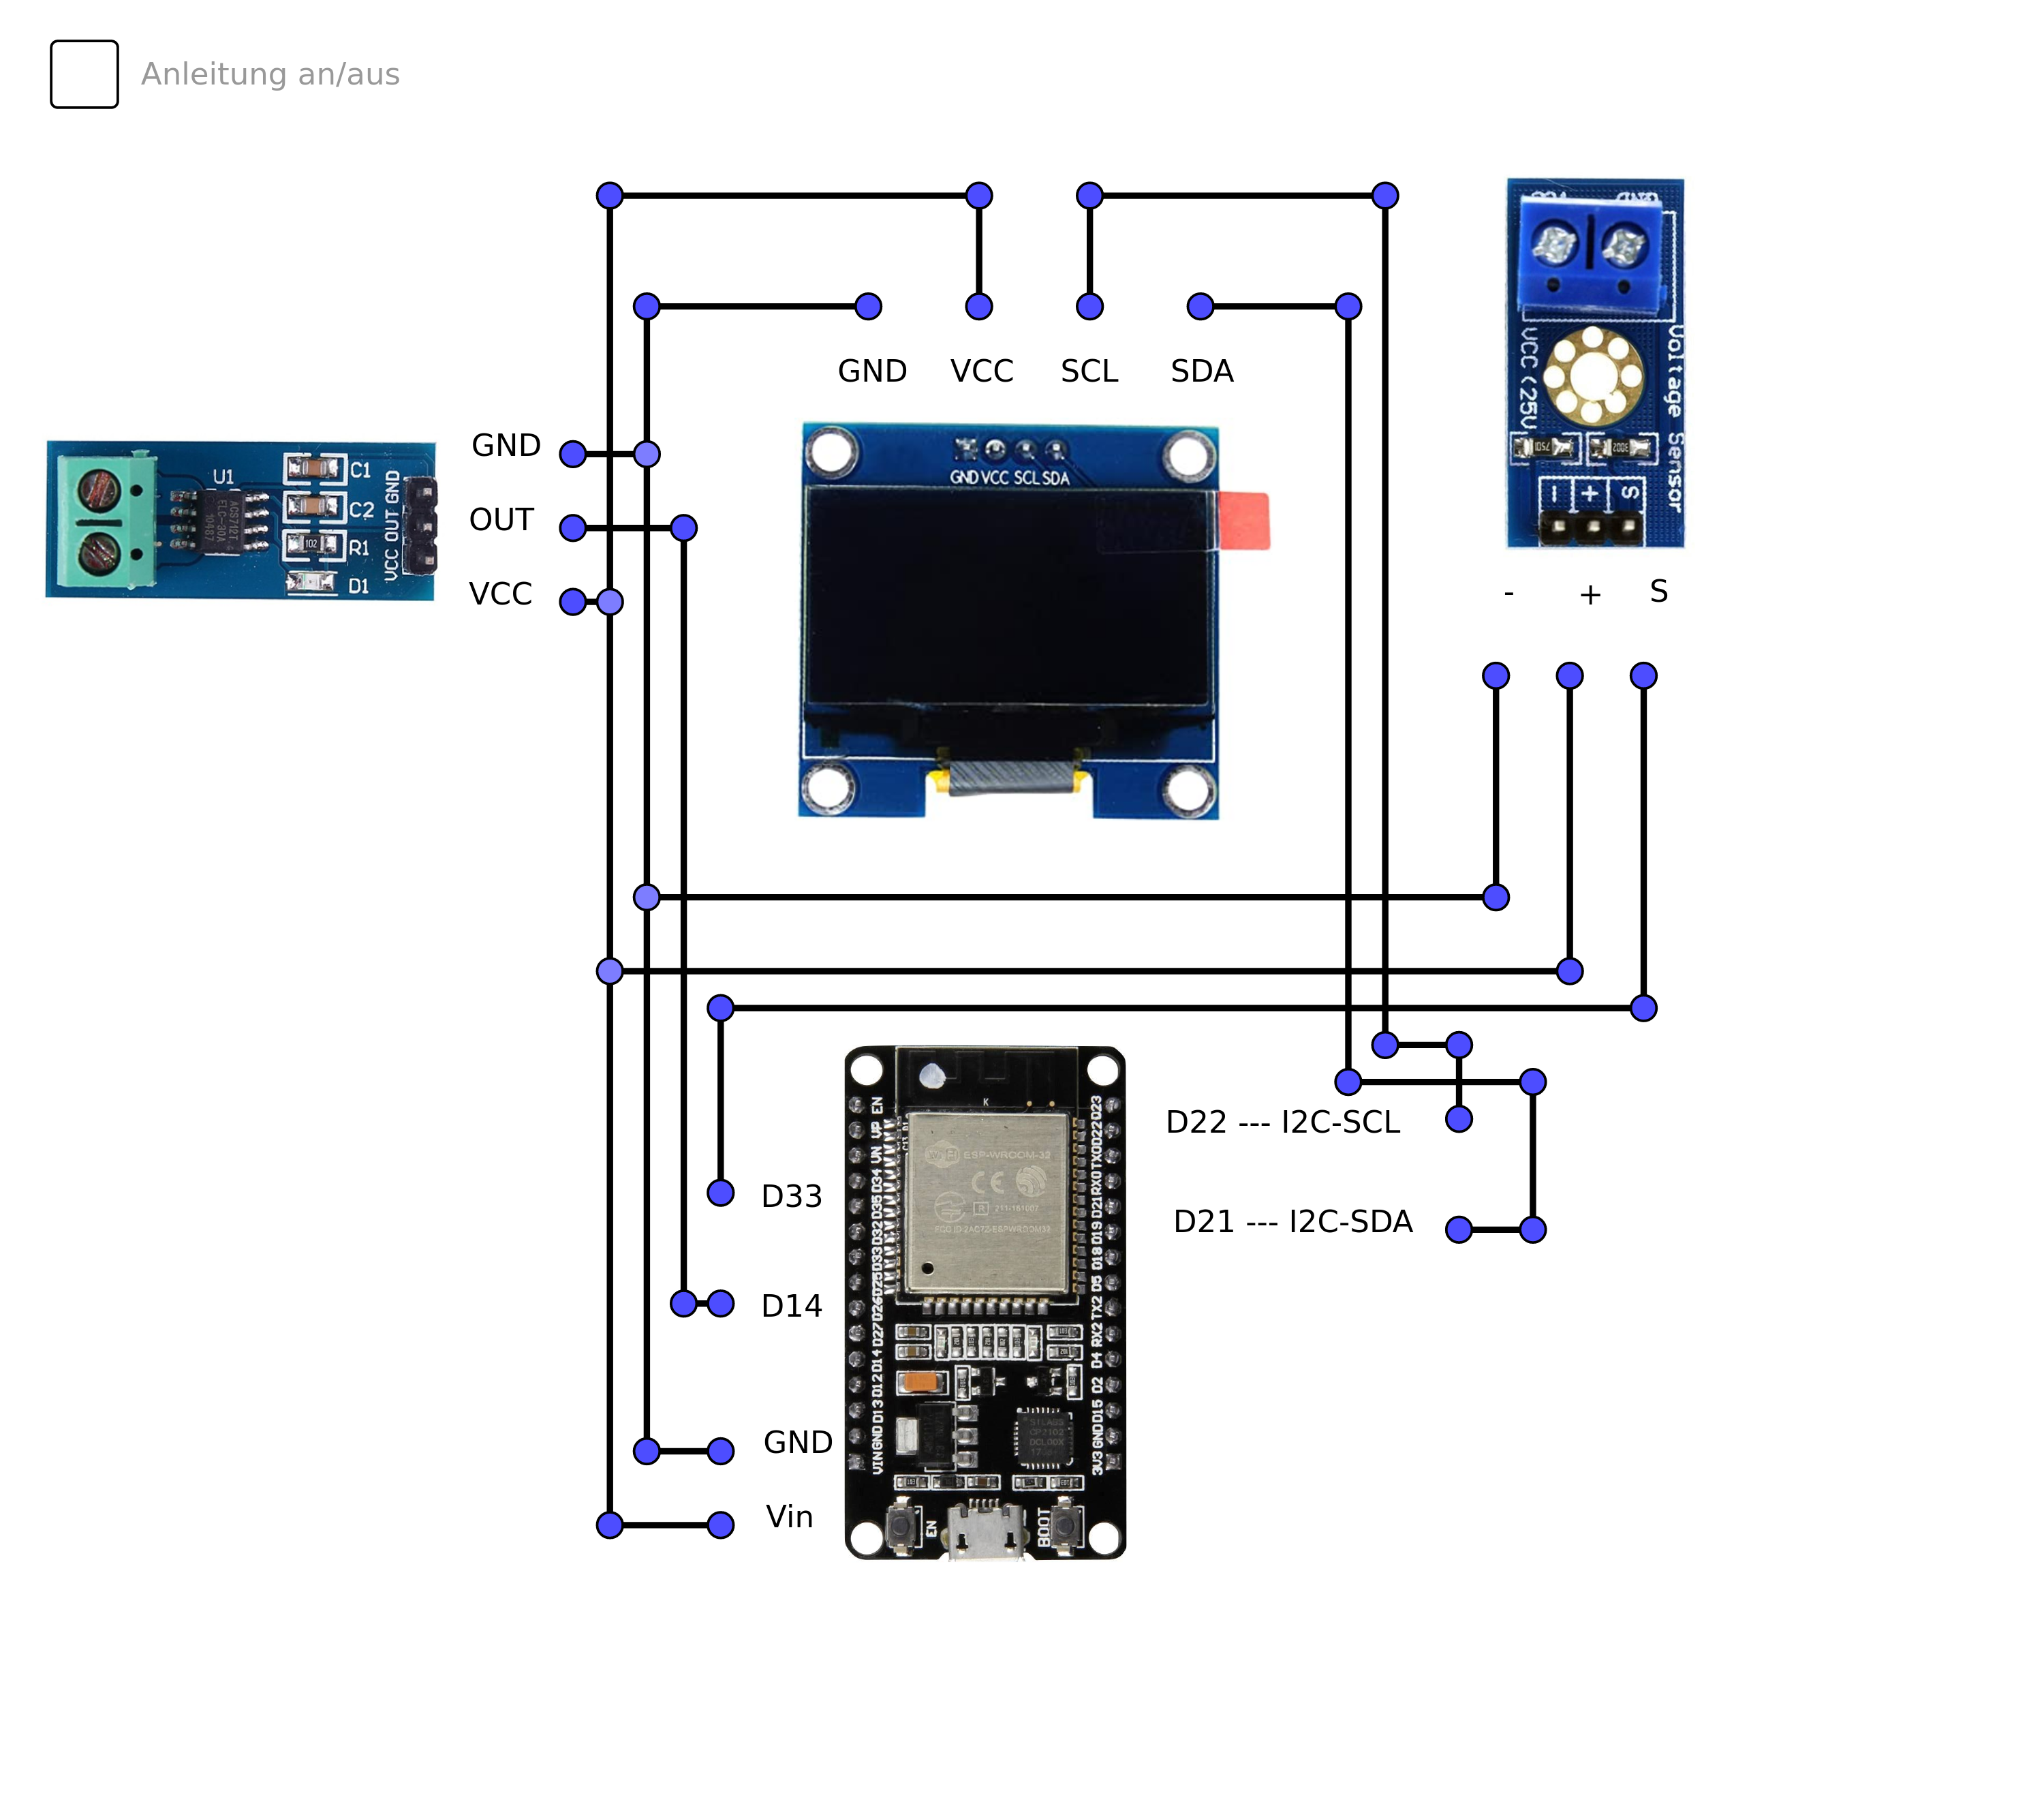
\includegraphics[width=1\linewidth]{Bilder/Schaltbilder/Monitoring_Schaltung.png}
			\caption{Schaltskizze der Monitoring Einheit}
			\label{fig:Monitoring Einheit}
		\end{figure}
		
		
		
		Bevor der Endzustand des Monitoring Systems festgelegt wurde auf nur zwei Sensoren waren es vier. Doch nach mehreren versuchen die Batteriespannung abzuklemmen wurde die Strom und Spannungsmessung der Batterie aufgegeben. Ein Kurzschluss hat leider eine alte Schaltung und einen Step-up Booster zerschossen. Deswegen ist es dabei geblieben nur den Strom und die Spannung des Solarmoduls zu messen. Diese erfolgen wie oben genannt mit einem ACS712 für den Strom und einem Spannungsmessmodul für die Spannung.

	\begin{figure}
		\centering
		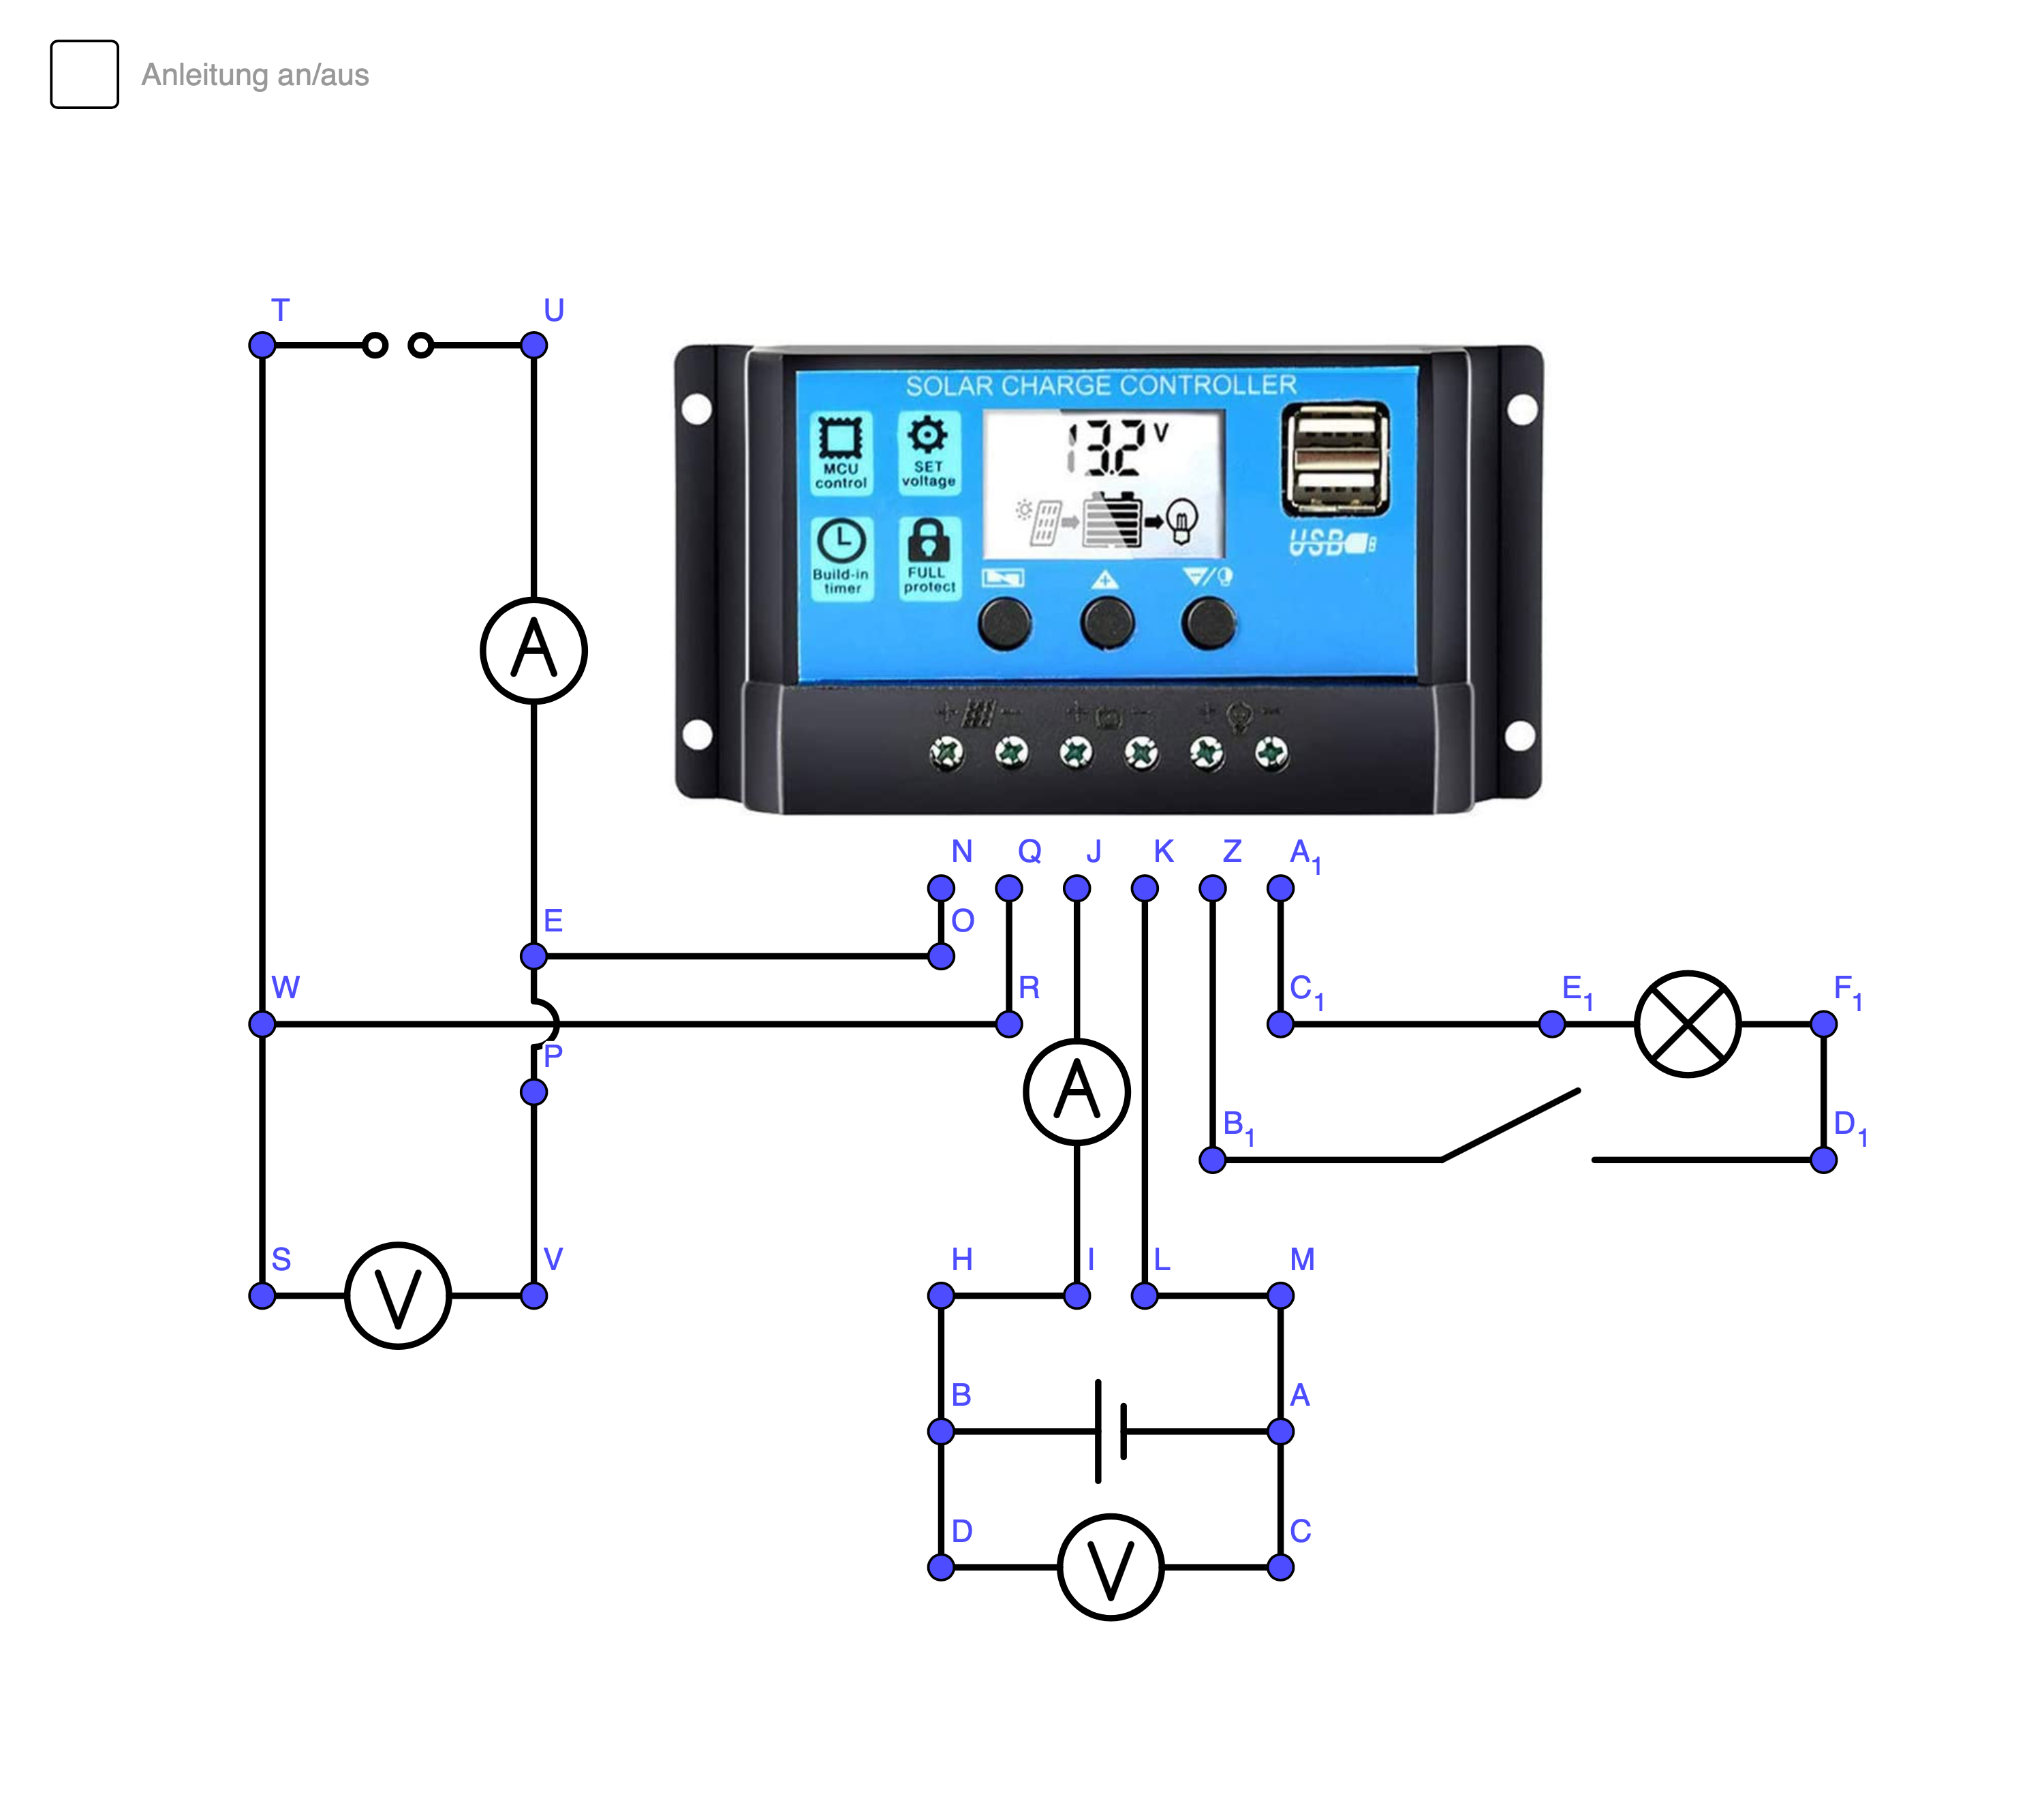
\includegraphics[width=1\linewidth]{Bilder/Schaltbilder/SchaltungAnlage.png}
		\caption{Schaltskizze der Solaranlage}
		\label{fig: Schaltskizze Solaranlage alt}
	\end{figure}
	
Durch den vorfall fällt natürlich die Strom-/Spaannungsmessung an der Batterie weg, sodass die Schaltskizze nun wie im folgenden Bild zu sehen aufgebaut ist.


	\begin{figure}
		\centering
		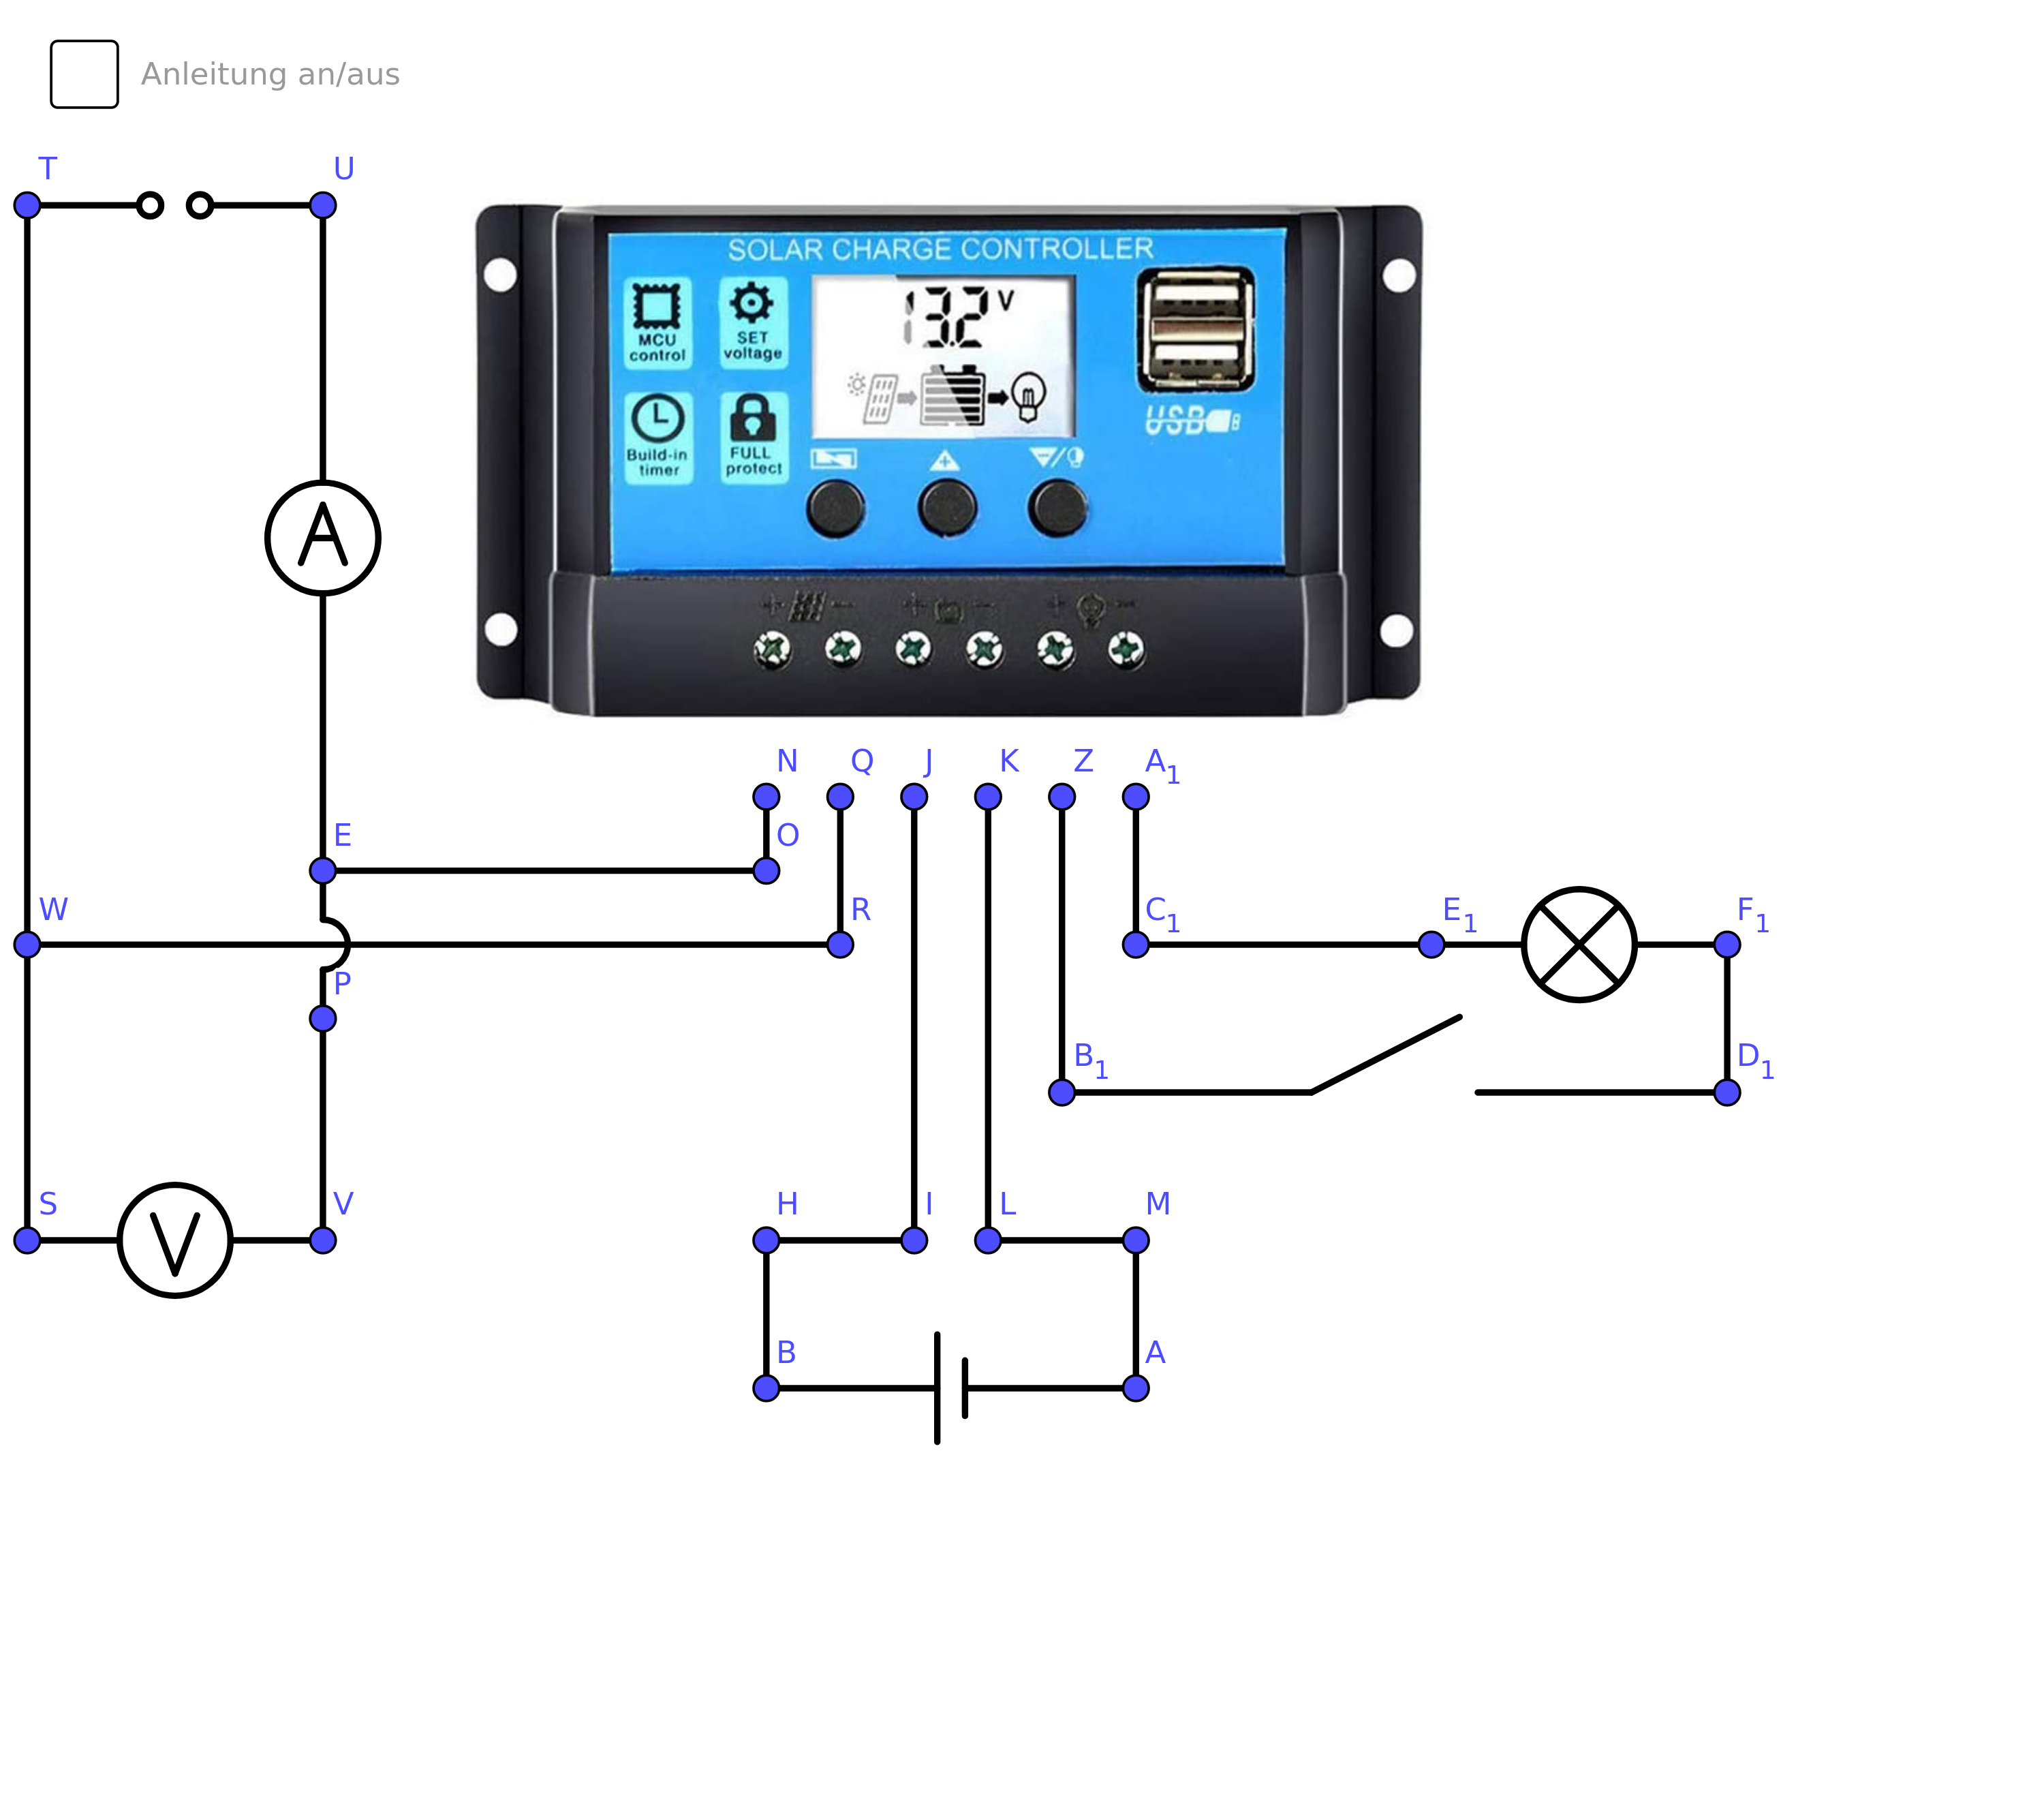
\includegraphics[width=1\linewidth]{Bilder/Schaltbilder/SchaltungOhneBatterieMessung.png}
		\caption{Schaltskizze der Solaranlage ohne Messung der Batterie}
		\label{fig: Schaltskizze Solaranlage neu}
	\end{figure}

Als Verbraucher fungieren zwei LED-Stäbe die in einem alten Laderegler verbaut sind. Die Anschlüsse der LED-Stäbe wurden nicht ausgebaut, da die Anschlusse einen neuen geeigneten Platz benötigt hätten. So sind sie sicher vor Zugbelastung und haben einen festen halt. 
		
				
%		\begin{figure}
%			\centering
%			\includegraphics[width=1\linewidth]{Bilder/Dokubilder/LadereglerAlt.jpg}
%			\caption{Verbraucher}
%			\label{fig:Verbraucher}
%		\end{figure}
	
		\begin{figure}
			\centering
			\includegraphics[width=1\linewidth]{Bilder/Dokubilder/Monitoring1.jpg}
			\caption{Monitoring mit Input Voltage}
			\label{fig:Monitoring1}
		\end{figure}
		
		\begin{figure}
			\centering
			\includegraphics[width=1\linewidth]{Bilder/Dokubilder/Monitoring2.jpg}
			\caption{Monitoring mit Output Voltage}
			\label{fig:Monitoring2}
		\end{figure}

%%%%%%%%%%%%%%%%%%%%%%%%%%%%%%%%%%%%%%%%%%%%%%%%%%%%%%%%%%%%%%%%%%%%%
\subsection{Elektrik}
		
		\begin{table}[]
		\begin{tabular}{|l|l|l|}
		\hline
  			  	& Solar  & Batterie \\ \hline
			$U_L$ & $21,2$ V & $12,78$ V  \\ \hline
			$I_K$ & $490$ mA & $108$ mA   \\ \hline 
		\end{tabular}
		\end{table}
		
		
		
%%%%%%%%%%%%%%%%%%%%%%%%%%%%%%%%%%%%%%%%%%%%%%%%%%%%%%%%%%%%%%%%%%%%%%
\subsection{Schaltung}

Die Schaltung des Monitoring Systems ist dem folgenden schaubild zu entnehmen.

		\begin{figure}
			\centering
			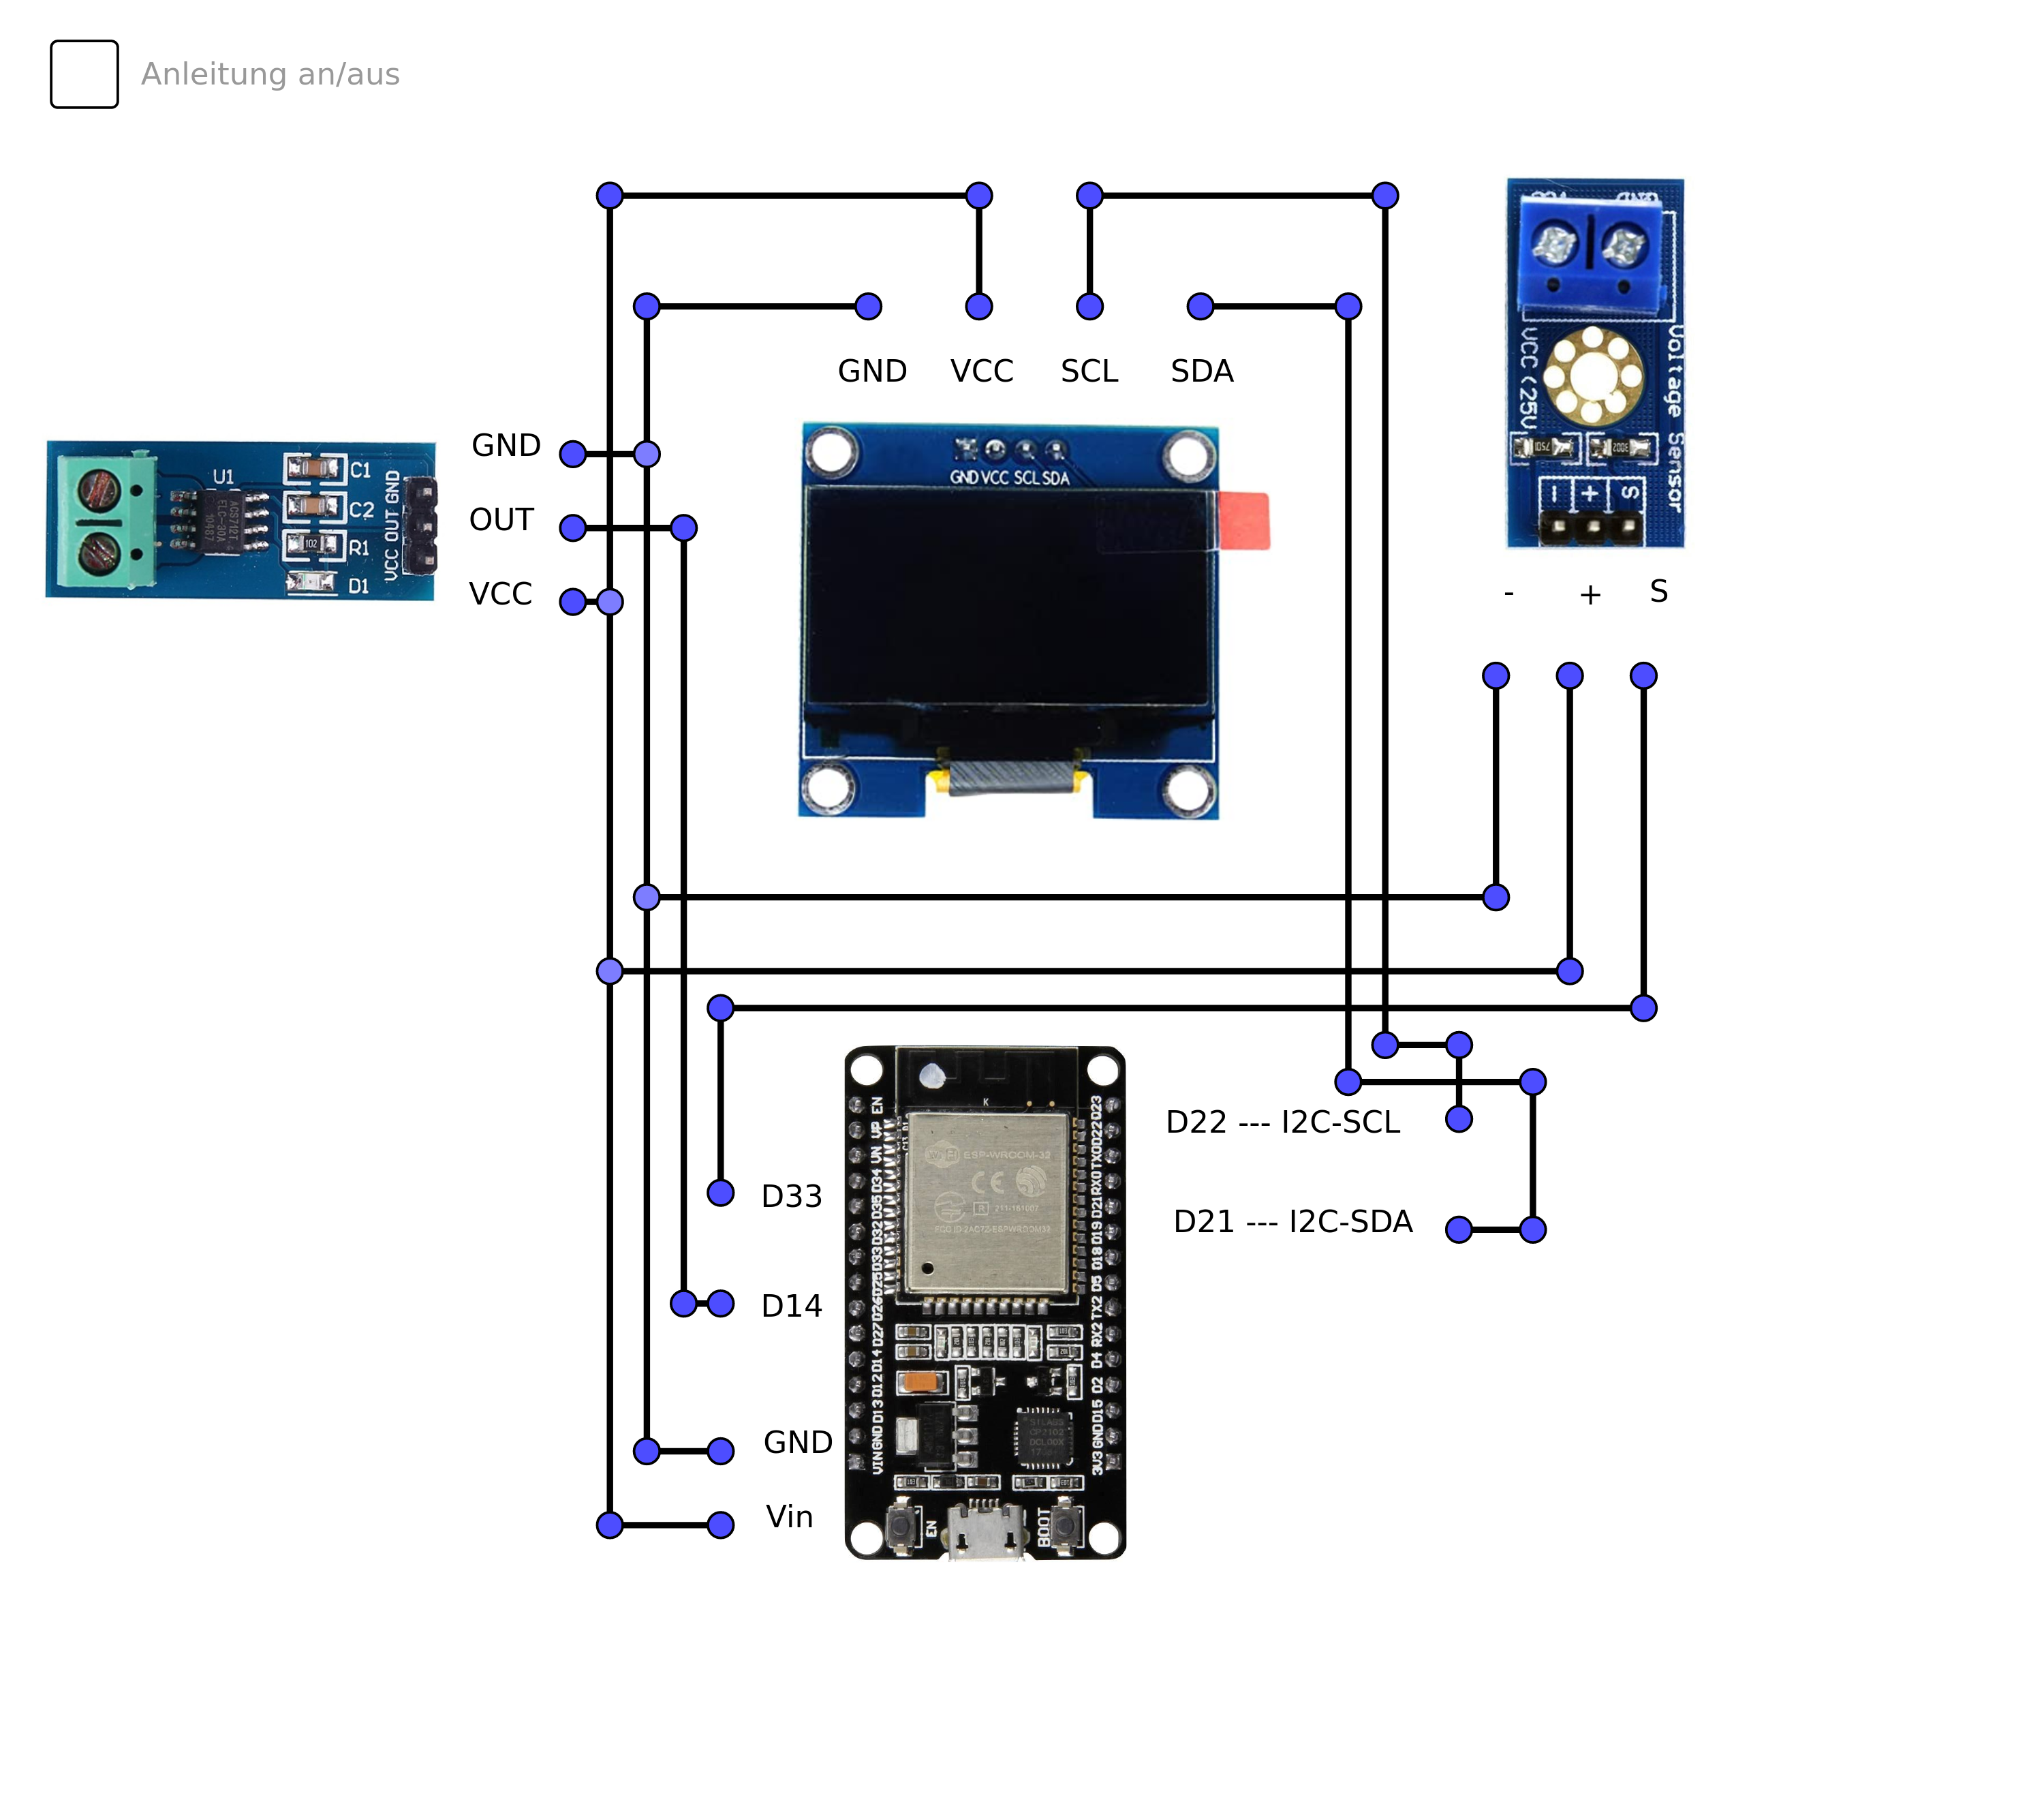
\includegraphics[width=1\linewidth]{Bilder/Schaltbilder/Monitoring_Schaltung.png}
			\caption{Schaltskizze der Monitoring Einheit}
			\label{fig:Monitoring Einheit}
		\end{figure}


%%%%%%%%%%%%%%%%%%%%%%%%%%%%%%%%%%%%%%%%%%%%%%%%%%%%%%%%%%%%%%%%%%%%%%
\subsection{code}

Der Programmcode besteht aus zwei Bestandteilen. Zum einen dem Sketch für den Arduino und zum anderen dem HTML-Code für den Webserver.

\begin{minted}{C}
String readVoltage() {
  return String(spannungsmessung());
}

String readCurrent() {
  return String(strommessung());
}

String calculatePower() {
  return String(leistungsBerechnung());
}
\end{minted}


%%%%%%%%%%%%%%%%%%%%%%%%%%%%%%%%%%%%%%%%%%%%%%%%%%%%%%%%%%%%%%%%%%%%%%
\subsection{Drahtlose Übertragung}

Um eine Solaranlage nutzbar zu gestalten bedarf es mehrere Einzelkomponenten die in einem Zusammenspiel arbeiten.

%%%%%%%%%%%%%%%%%%%%%%%%%%%%%%%%%%%%%%%%%%%%%%%%%%%%%%%%%%%%%%%%%%%%%%
\subsection{Laderegler - Bestandteile}

Ein Laderegler unterstütz den optimalen Ladevorgang einer Batterie. Der Laderegler ist an das Solarmodul geschlossen, der Batterie und an einen Verbraucher.



%%%%%%%%%%%%%%%%%%%%%%%%%%%%%%%%%%%%%%%%%%%%%%%%%%%%%%%%%%%%%%%%%%%%%%%%%%%%%%%%%%%%%%%%%%%%%%%%%%%%%%%%%%%%%%%%%%%%%%%%%%%%%%%%%%%%%%%%%%%%
\section{Fazit und Ausblick}
In Zukunft ist es auch möglich über eine Relaisschaltung Verbraucher zuzuschalten.

In Zukunft möchte ich gerne ein Mppt-Regler bauen der drei Zustände besitzt. Den "Bulk-Modus" der eine konstante Stromstärke liefert um die Batterie bis auf 80\% zu laden (ohne rücksicht auf die Spannung zu nehmen). Ab einer bestimmten Spannung der Batterie soll der nächste Zustand einsetzen "Absorption". Hier bleibt die Spannung durch den Controller konstant, die Stromstärke nicht mehr, diese fällt mit dem Ladezustand der Batterie (nahe 100\%). Dann sobald die Batterie die restlichen 20\% geladen hat soll der Controller in den "Float"-Modus. In diesem Zustand reduziert der Controller die Spannung auf einen festgesetzten Wert und der Stromfluss reduziert sich auf einen Wert kleiner als 1\% der Batterie Kapazität. Dadurch kann die Batterie unendlich lange voll geladen bleiben. Ein Bild dieser Idee sieht man auf der folgenden Abbildung\ref{fig:MPPT Solar Charger Prototype}.

\begin{figure}
			\centering
			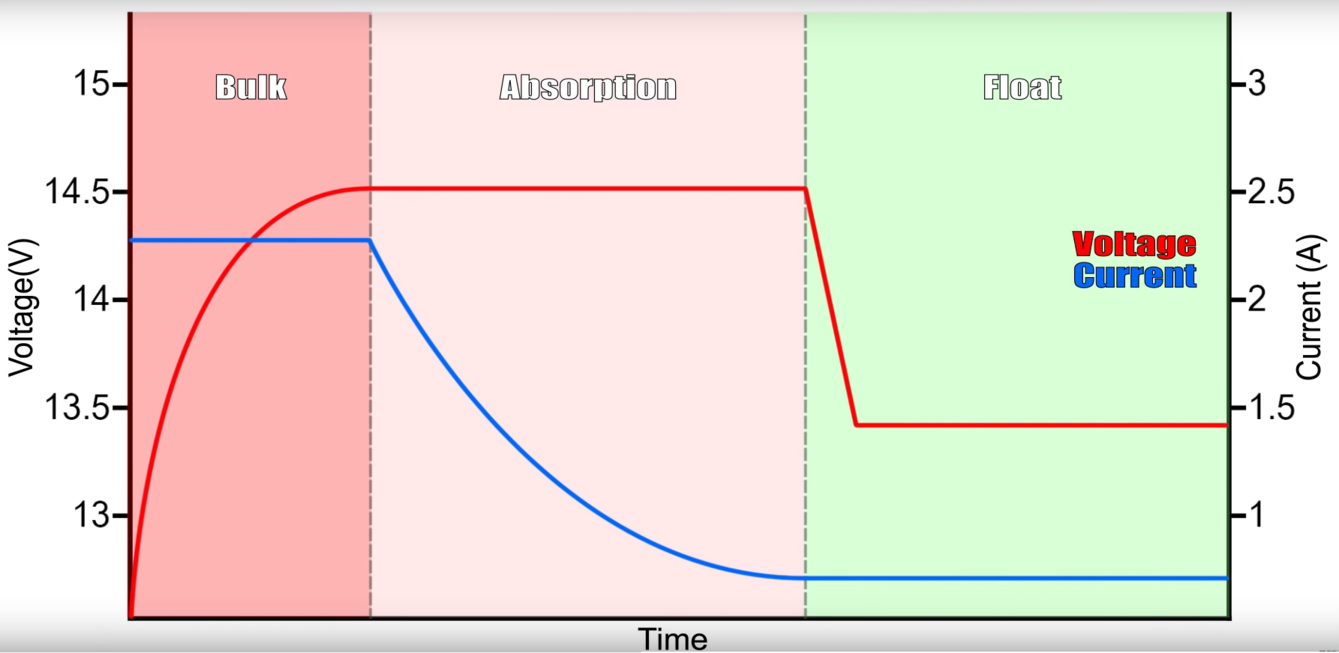
\includegraphics[width=1\linewidth]{Bilder/Dokubilder/ChargeController1.png}
			\caption{Ladekurve der Mppt-Controller Idee}
			\label{fig:MPPT Solar Charger Prototype}
		\end{figure}


Ich habe einen solchen Versuch gestartet. Nach einigen durchgebrannten Schaltungen und fehlenden Teilen habe ich diesen Versuch eingefroren. 


\begin{figure}
		\centering
		\includegraphics[width=1\linewidth]{Bilder/Dokubilder/Anlage.jpg}
		\caption{Anlage in Konstruktion}
		\label{fig:Solaranlage}
	\end{figure}


\section{Anhang}

\lstinputlisting[language=C++,
basicstyle=\scriptsize,linerange={1,17-42},
numbers=left,numberstyle=\tiny,stepnumber=2,numbersep=5pt,
frame=single, framerule=1pt
]{code/monitoring.ino}

\lstinputlisting[language=HTML,
basicstyle=\scriptsize,linerange={1,17-42},
numbers=left,numberstyle=\tiny,stepnumber=2,numbersep=5pt,
frame=single, framerule=1pt
]{code/data/index.html}

\end{document}
